\chapter{Les R\^oles et Les Utilisateurs}\label{chap:utilisateurs}
\index{types de \roles}

\utilisateurs: \lienadmin, \liencaissier, \lienmagasinier, \lienpatron.\\

\chapintro{Ce chapitre d\'ecrit les diff\'erents types d'utilisateurs de
\yeren: \admin, \magasinier, \caissier, et \patron.}

\nxsection{Introduction}\label{sec:utilisateurs-introduction}

\yeren maintient les donn\'ees suivantes pour chaque utilisateur:
\begin{enumerate}[1)]
	\item l'\'email \optionel
	\item la bo\^ite postale
	\item le date de naissance \optionel
	\item le lieu de naissance \optionel
	\item la localisation (le site de l'entreprise o\`u l'employ\'e
	      est en fonction). Cette valeur ne peut \^etre \'edit\'ee.
	      Sa valeur est automatiquement remplie \`a partir de la
	      license d'installation.
	\item le nom
	\item le num\'ero de t\'el\'ephone 1 \optionel
	\item le num\'ero de t\'el\'ephone 2 \optionel
	\item le pays \optionel
	\item le pr\'enom	
	\item la province / \'etat
	\item le r\^ole dans \yeren (\admin, \magasinier, \caissier, ou \patron)
	\item le titre (Dr., Me., Mlle, Mme, Mr, Pr., Prof.)
	\item la ville \optionel
\end{enumerate}

\newpage

\nxsection{Le r\^ole ''Administrateur''}\label{sec:utilisateurs-ladministrateur}
\index{administrateur}
\index{LAdministrateur}

La figure~\ref{fig:fenetre-principale-admin} illustre la
fen\^etre d'acceuil d'un utilisateur avec le \role \admin,
apr\`es qu'il se soit enregistr\'e dans \yeren.\\

\begin{figure}[!htbp]
\centering
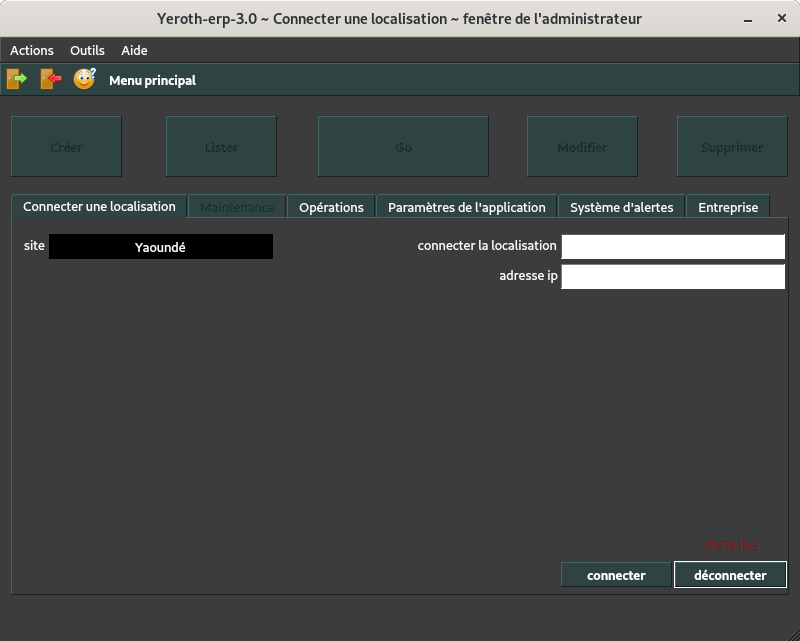
\includegraphics[scale=0.63]{images/yeroth-fenetre-administrateur.png}
\caption{La fen\^etre d'acceuil d'un administrateur.}
\label{fig:fenetre-principale-admin}
\end{figure}

Un utilisateur avec le \role "\admin" assume les
t\^aches de cr\'eer et de maintenir les objets suivants:
\begin{enumerate}[1)]
	\item les alertes (sur une p\'eriode de temps, ou sur une quantit\'e en stock)
	%\item les bons de commande
	\item les cat\'egories d'articles
	\item les clients
	\item les comptes utilisateurs
	\item les fournisseurs				
	\item les localisations (une localisation est un site de
	      l'entreprise o\`u se trouve un ou plusieurs stocks).\\   
\end{enumerate}

\newpage

\nxsection{Le r\^ole ''Manager''}\label{sec:utilisateurs-lepatron}
\index{patron}
\index{LePatron}

La figure~\ref{fig:yeren-fenetre-patron} illustre la fen\^etre
d'acceuil d'un utilisateur avec le \role \patron, 
apr\`es qu'il se soit enregistr\'e dans \yeren.\\

\begin{figure}[!htbp]
\centering
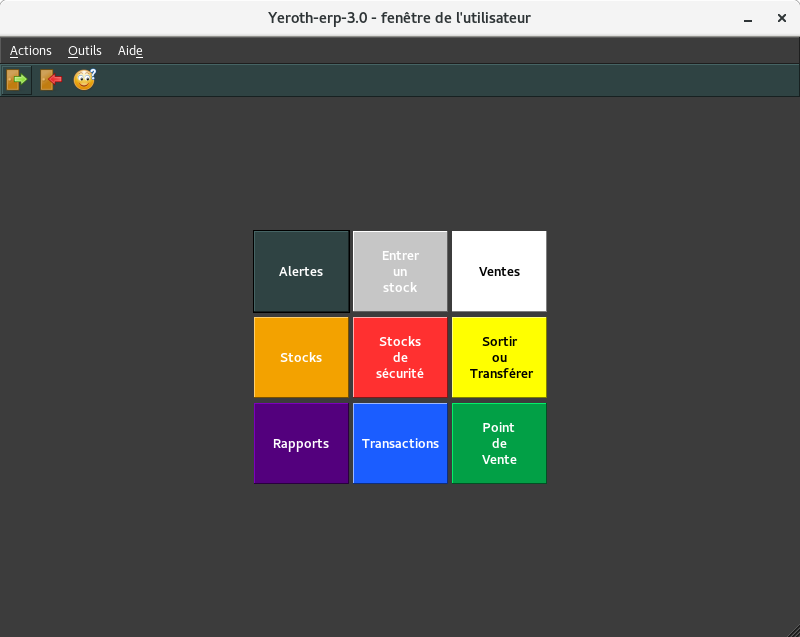
\includegraphics[scale=0.63]{images/yeren-fenetre-patron.png}
\caption{La fen\^etre d'acceuil d'un ''manager''}
\label{fig:yeren-fenetre-patron}
\end{figure}

Un utilisateur de \yeren avec le \role "\patron" a
acc\`es \`a toutes les fonctionalit\'es de \yeren. Il
cumule les t\^aches de d'administrateur, de magasinier,
et de caissier.

Le \role \patron est le seul \`a donner acc\`es aux
informations des ventes dans leurs totalit\'es, ainsi
qu'\`a la g\'en\'eration et \`a la consultation des
rapports commerciaux.

Le \role \patron est le seul \`a pouvoir consulter toutes
les alertes re\c{c}ues par les autres utilisateurs, et
\`a pouvoir les supprimer.

\newpage

\nxsection{Le r\^ole ''GestionaireDeStocks''}\label{sec:utilisateurs-gestionairedestocks}
\index{gestionaire de stocks}
\index{GestionaireDeStocks}

La figure~\ref{fig:yeren-fenetre-gestionairedestocks} illustre
la fen\^etre d'acceuil d'un utilisateur avec le \role \gestionairedestocks, 
apr\`es qu'il se soit enregistr\'e dans \yeren.\\

\begin{figure}[!htbp]
\centering
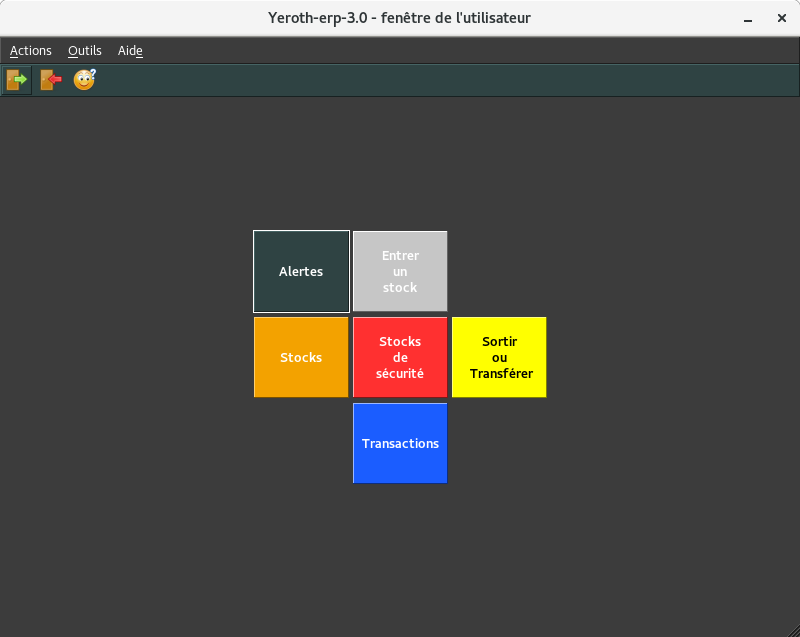
\includegraphics[scale=0.63]{images/yeren-fenetre-gestionairedestocks.png}
\caption{La fen\^etre d'acceuil d'un gestionaire de stocks}
\label{fig:yeren-fenetre-gestionairedestocks}
\end{figure}

\newpage

\nxsection{Le r\^ole ''Magasinier''}\label{sec:utilisateurs-lemagasinier}
\index{magasinier}
\index{LeMagasinier}

La figure~\ref{fig:yeren-fenetre-magasinier} illustre
la fen\^etre d'acceuil d'un utilisateur avec le
\role \magasinier, apr\`es qu'il se soit enregistr\'e
dans \yeren.\\

\begin{figure}[!htbp]
\centering
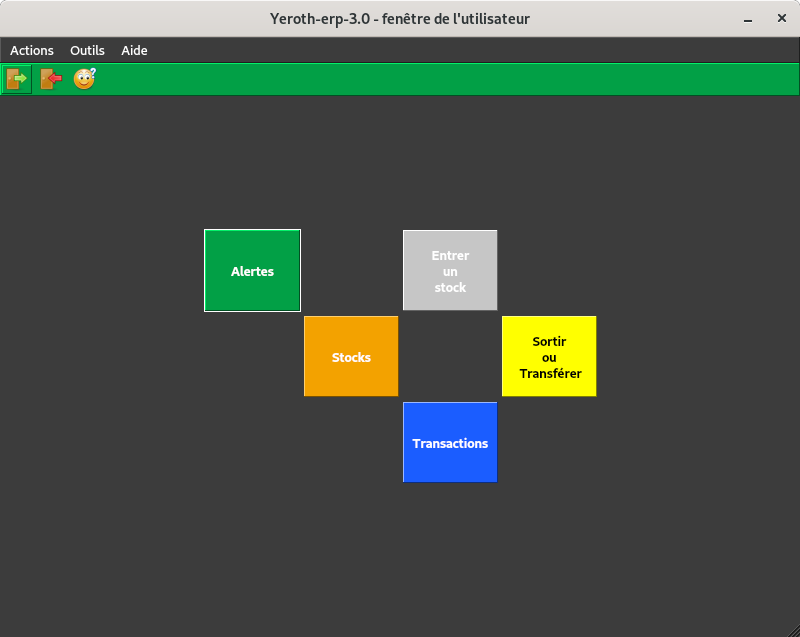
\includegraphics[scale=0.63]{images/yeren-fenetre-magasinier.png}
\caption{La fen\^etre d'acceuil d'un magasinier.}
\label{fig:yeren-fenetre-magasinier}
\end{figure}

Un utilisateur de \yeren avec le \role "\magasinier" assume les
t\^aches suivantes:
\begin{enumerate}[1)]
	\item lister des stocks
	\item modifier un stock
	\item rechercher des articles / stocks
	\item rechercher des transactions 
		(sorties de stocks ou transferts de stocks)
	\item sortir des articles / stocks
	\item supprimer un stock
	\item transf\'erer un stock
	\item visualiser des transactions
	(sorties de stocks ou transferts de stocks).\\
\end{enumerate}

\magasinier n'a pas acc\`es aux fonctions
\bouton{Administration}, \bouton{Ventes},
\bouton{Rapports}, et \bouton{Vendre}.

On remarque sur la Figure~\ref{fig:yeren-fenetre-magasinier}
que les boutons \bouton{Administration}, \bouton{Ventes},
\bouton{Rapports}, et \bouton{Vendre} sont d\'esactiv\'es.
	
\newpage

\nxsection{Le r\^ole ''Caissier''}\label{sec:utilisateurs-lecaissier}
\index{caissier}
\index{LeCaissier}

La figure~\ref{fig:fenetre-principale-caissier} illustre la
fen\^etre d'acceuil d'un utilisateur avec le \role \caissier,
apr\`es qu'il se soit enregistr\'e dans \yeren.\\

\begin{figure}[!htbp]
\centering
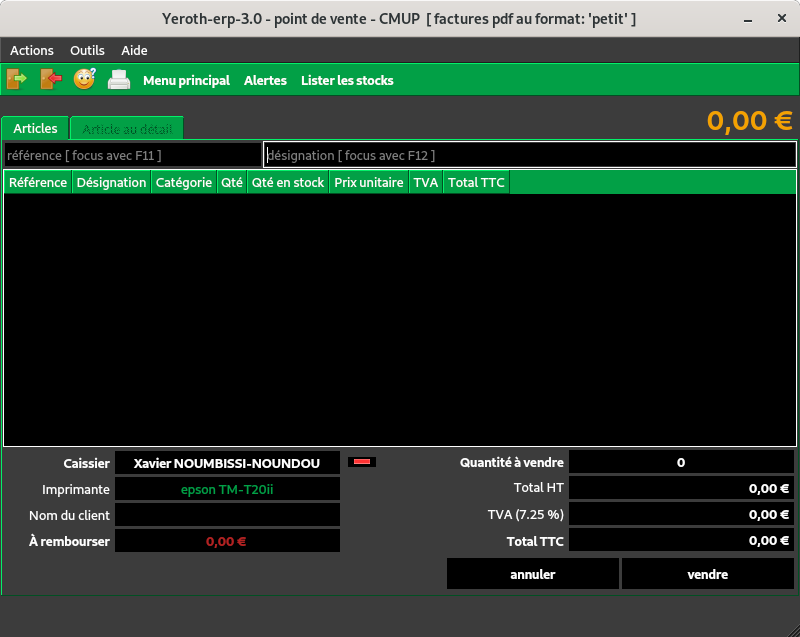
\includegraphics[scale=0.63]{images/yeren-fenetre-caissier.png}
\caption{La fen\^etre d'acceuil d'un caissier.}
\label{fig:fenetre-principale-caissier}
\end{figure}

Un utilisateur de \yeren avec le \role "\caissier" assume
les t\^aches suivantes:
\begin{enumerate}[1)]
	\item lister les stocks \`a partir de l'interface de vente	
	\item visualiser une facture proforma		
	\item imprimer une facture proforma
	\item vendre un ou plusieurs stocks (ou articles).\\
\end{enumerate}
